\documentclass{beamer}
\usepackage[utf8]{inputenc}
\usepackage{physics}
\usepackage[english,greek]{babel}
\usepackage{alphabeta}
\usepackage{amsmath, amssymb, amsfonts}
\usepackage{tikz, caption, subfig, comment, multicol, xcolor, tikz-feynman, tensor, graphics, graphicx, slashed, xfrac, biblatex, braket, siunitx, multirow, multicol}


\addbibresource{references.bib}
\usetheme{Madrid}
\usecolortheme{default}


\title[\href{https://summerstudent.web.cern.ch/home}{CERN Summer Student Programme 2023}]
{     
      New kinematic weighting algorithm for $CP$ asymmetries in charm decays
}
\setbeamerfont{footnote}{size=\tiny}
\setbeamerfont{caption}{size=\tiny}

\author[\href{https://github.com/GiorgosChr}{Georgios CHristou}]
{Georgios Christou
\\
Supervisors: Dr.\@ Federico Betti, Prof.\@ Angelo Carbone}

\institute[]
{
      LHCb Collaboration
}

\date{August 26, 2023}

% \logo{
\includegraphics[height=0.7cm]{../.images/Lhcb-logo-new.svg.png}}
\logo{\href{https://lhcb.web.cern.ch/}{
\includegraphics[height=0.7cm]{../.images/Lhcb-logo-new.svg.png}}}


\AtBeginSection[]{
  \begin{frame}
    \tableofcontents[currentsection]
  \end{frame}
}


\begin{document}
\selectlanguage{english}
\frame{\titlepage}
\begin{frame}
      \tableofcontents
\end{frame}

\section{Introduction}
\subsection{Asymmetries at the LHCb}


\begin{frame}
      \frametitle{\insertsubsectionhead}
      We are interested in the following charm decays and the asymmetries that occur
      \begin{eqnarray*}
            & D^{\star \pm} \to D^0 \pi^{\pm} \nonumber\\
            &D^0\to K^-K^+ \text{ or } D^0\to \pi^-\pi^+
      \end{eqnarray*}
      \textbf{At the LHCb we observe:}
      \begin{itemize}
            \item $CP$ asymmetries $\rightarrow$ matter and antimatter differences
            \item Detection asymmetries $\rightarrow$ detection of soft pions $(\pi^\pm_s)$
      \end{itemize}
\end{frame}

\begin{frame}
      \frametitle{\insertsubsectionhead}
      \begin{figure}
            \centering
            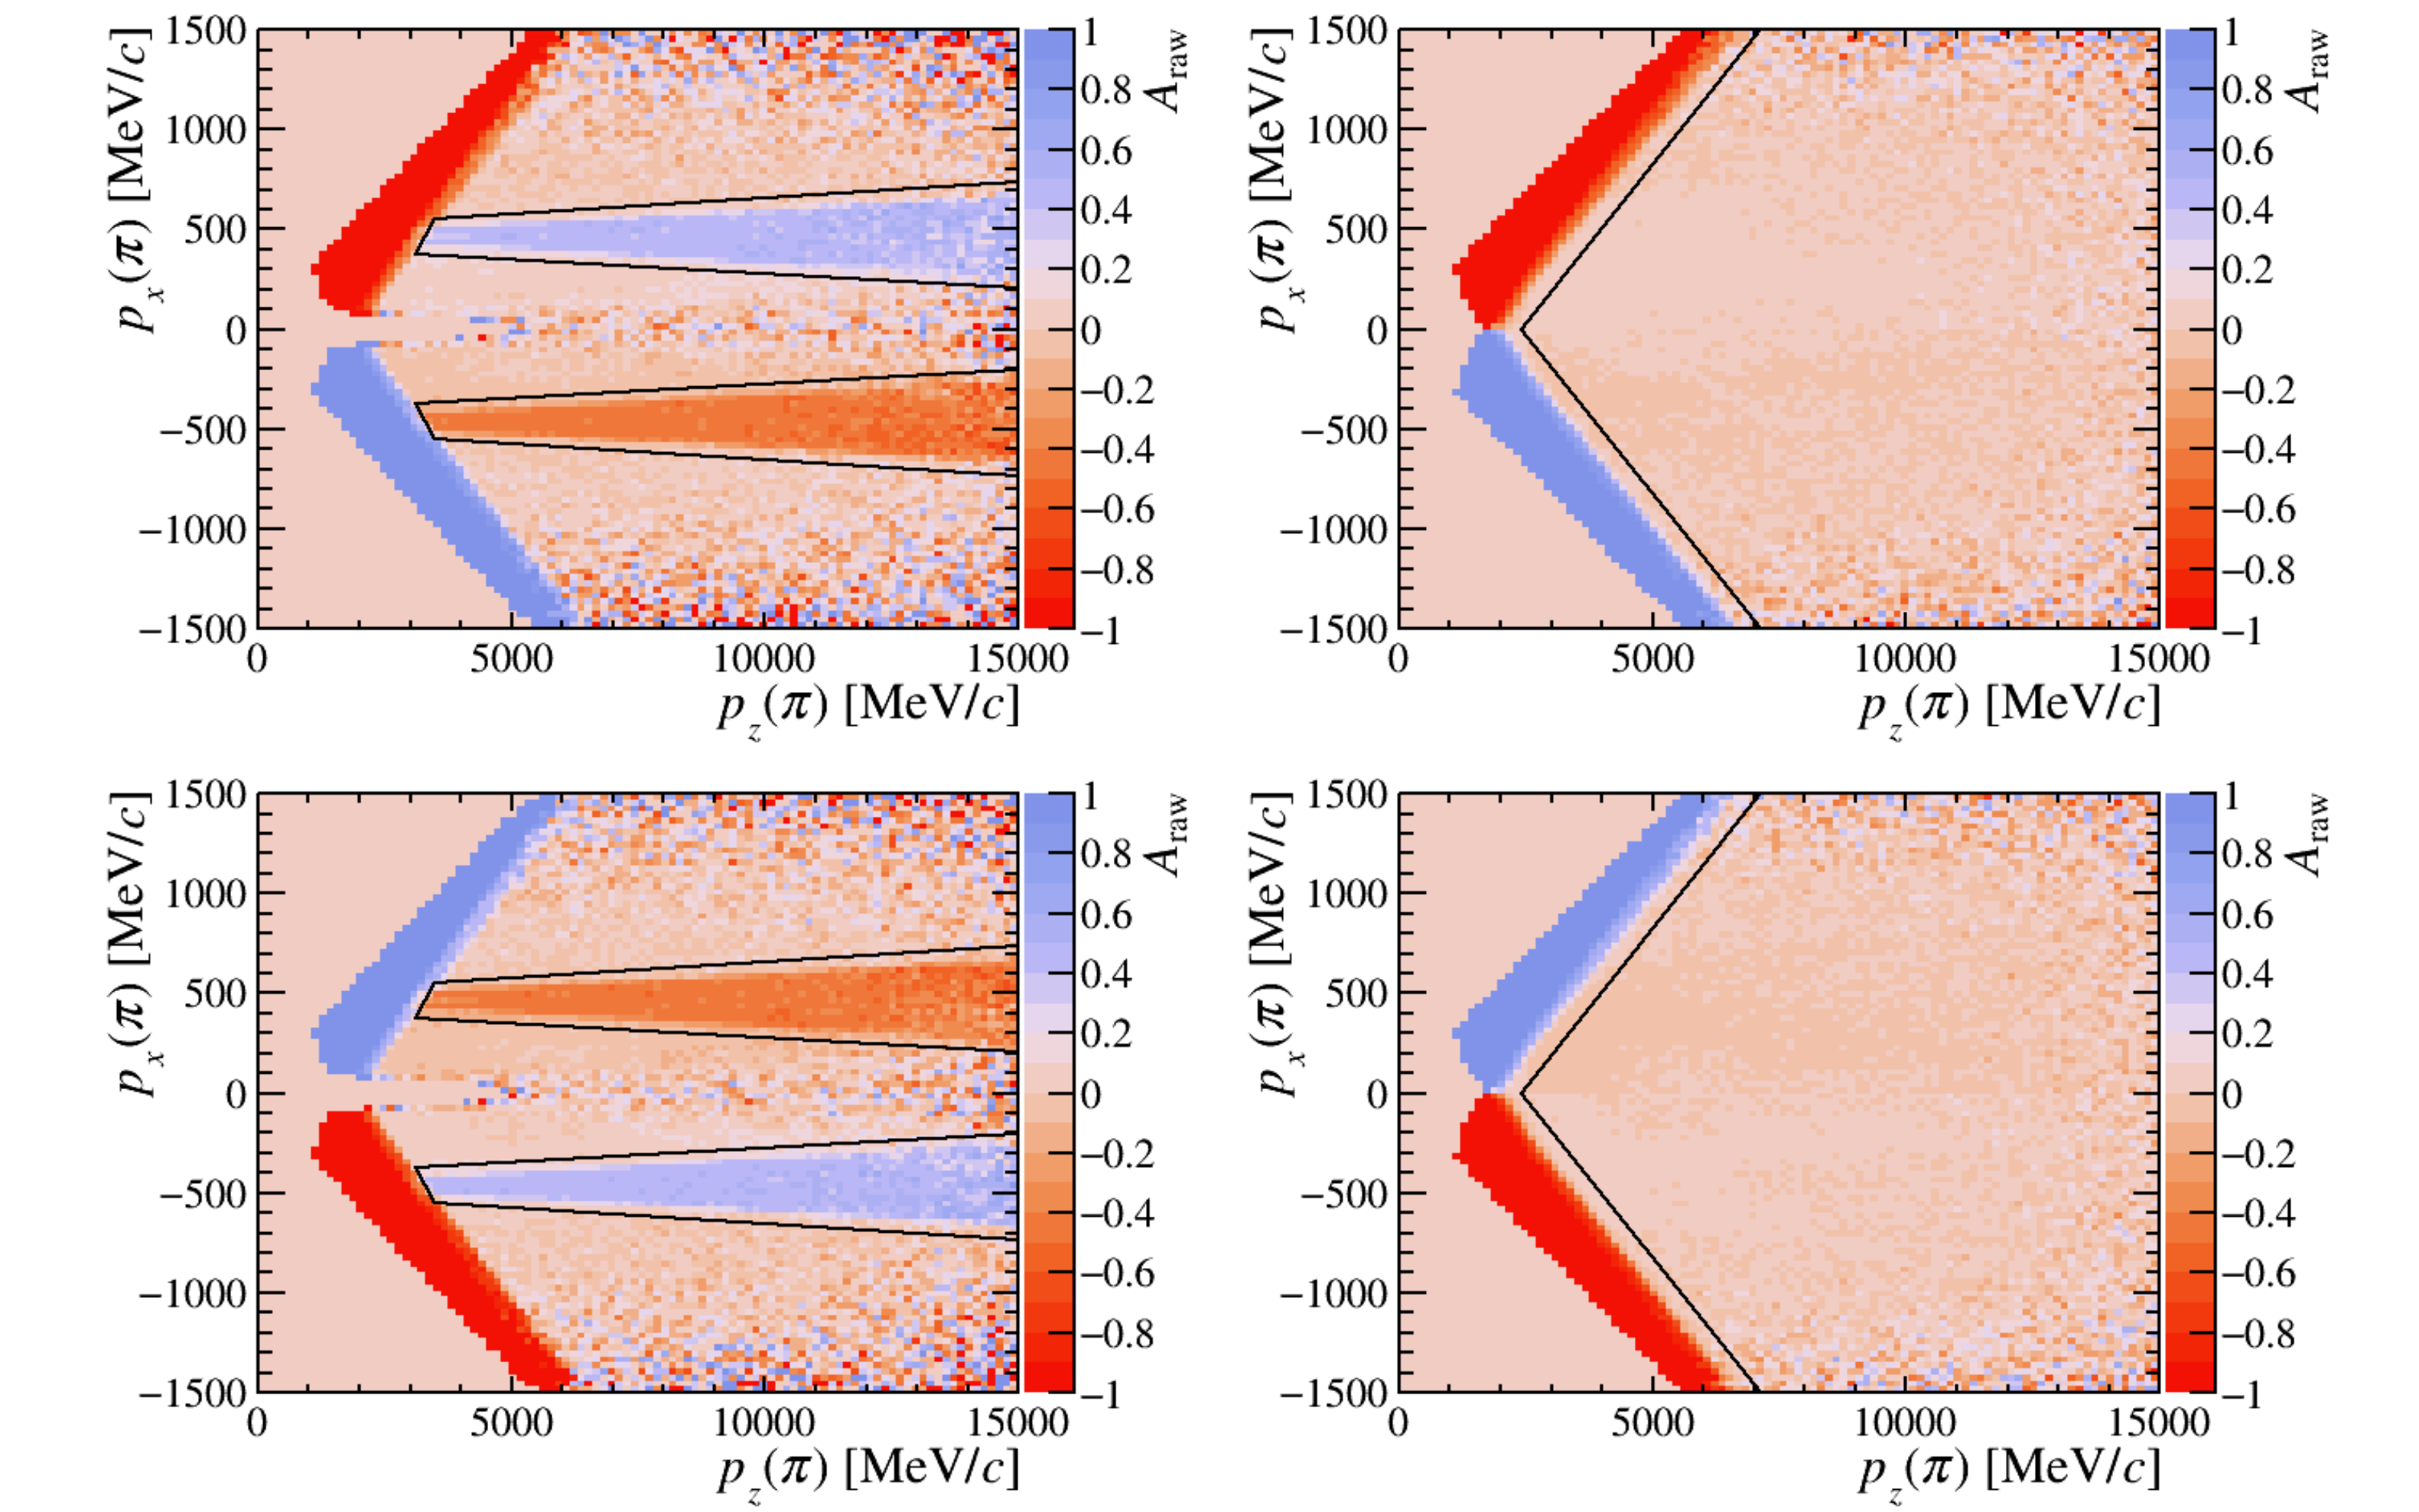
\includegraphics[width = 0.8\textwidth]{Figures/FedericoPlot.png}
            \caption{Asymmetries associated with certain kinematic regions of the soft pion. Credit: Federico Betti.}
      \end{figure}
\end{frame}

\begin{frame}
      \frametitle{\insertsubsectionhead}
      \textbf{How do we calculate asymmetries?}

      \begin{itemize}
      \item We can calculate the total number of positive and negative soft pions
      \end{itemize}
      \begin{equation*}
            A_\text{total} = \frac{N_+ - N_-}{N_+ + N_-}
      \end{equation*}
      \begin{itemize}
            \item We can also estimate the total asymmetry
      \end{itemize}
      \begin{equation*}
            A_\text{total} = \frac{A_{CP} + A_D}{1 + A_{CP} A_D}
      \end{equation*}
      We are interested in $\Delta A_\text{total} = A_\text{total}^{KK} - A_\text{total}^{\pi\pi}$
\end{frame}
\subsection{The weighting function}
\begin{frame}
      \frametitle{\insertsubsectionhead}
      \begin{itemize}
            \item We introduce the weighting function
      \end{itemize}
      \begin{equation*}
            Q(\vec{p}_{D^\star}, \vec{p}_{\pi_s}) \simeq \frac{\Gamma_{D^0}^{\pi\pi}(\vec{p}_{D^\star} - \vec{p}_{\pi_s}) + \Gamma_{\bar{D}^0}^{\pi\pi}(\vec{p}_{D^\star} - \vec{p}_{\pi_s})}{\Gamma_{D^0}^{KK}(\vec{p}_{D^\star} - \vec{p}_{\pi_s}) + \Gamma_{\bar{D}^0}^{KK}(\vec{p}_{D^\star} - \vec{p}_{\pi_s})}
    \end{equation*}
    \begin{itemize}
      \item We equalize $D^0\to K^- K^+$ and $D^0\to \pi^- \pi^+$ kinematic distributions
      \item The detection asymmetries should cancel out and $\Delta A_\text{total} = \Delta A_{CP}$
    \end{itemize}
\end{frame}

\section{RapidSim}
\subsection{Injecting detection asymmetry}
\begin{frame}
      \frametitle{\insertsubsectionhead}
      \begin{itemize}
            \item We inject $CP$ and detection asymmetries to the RapidSim data
      \end{itemize}
      \begin{columns}
            \column{0.5\textwidth}
                  \begin{figure}
                        \centering
                        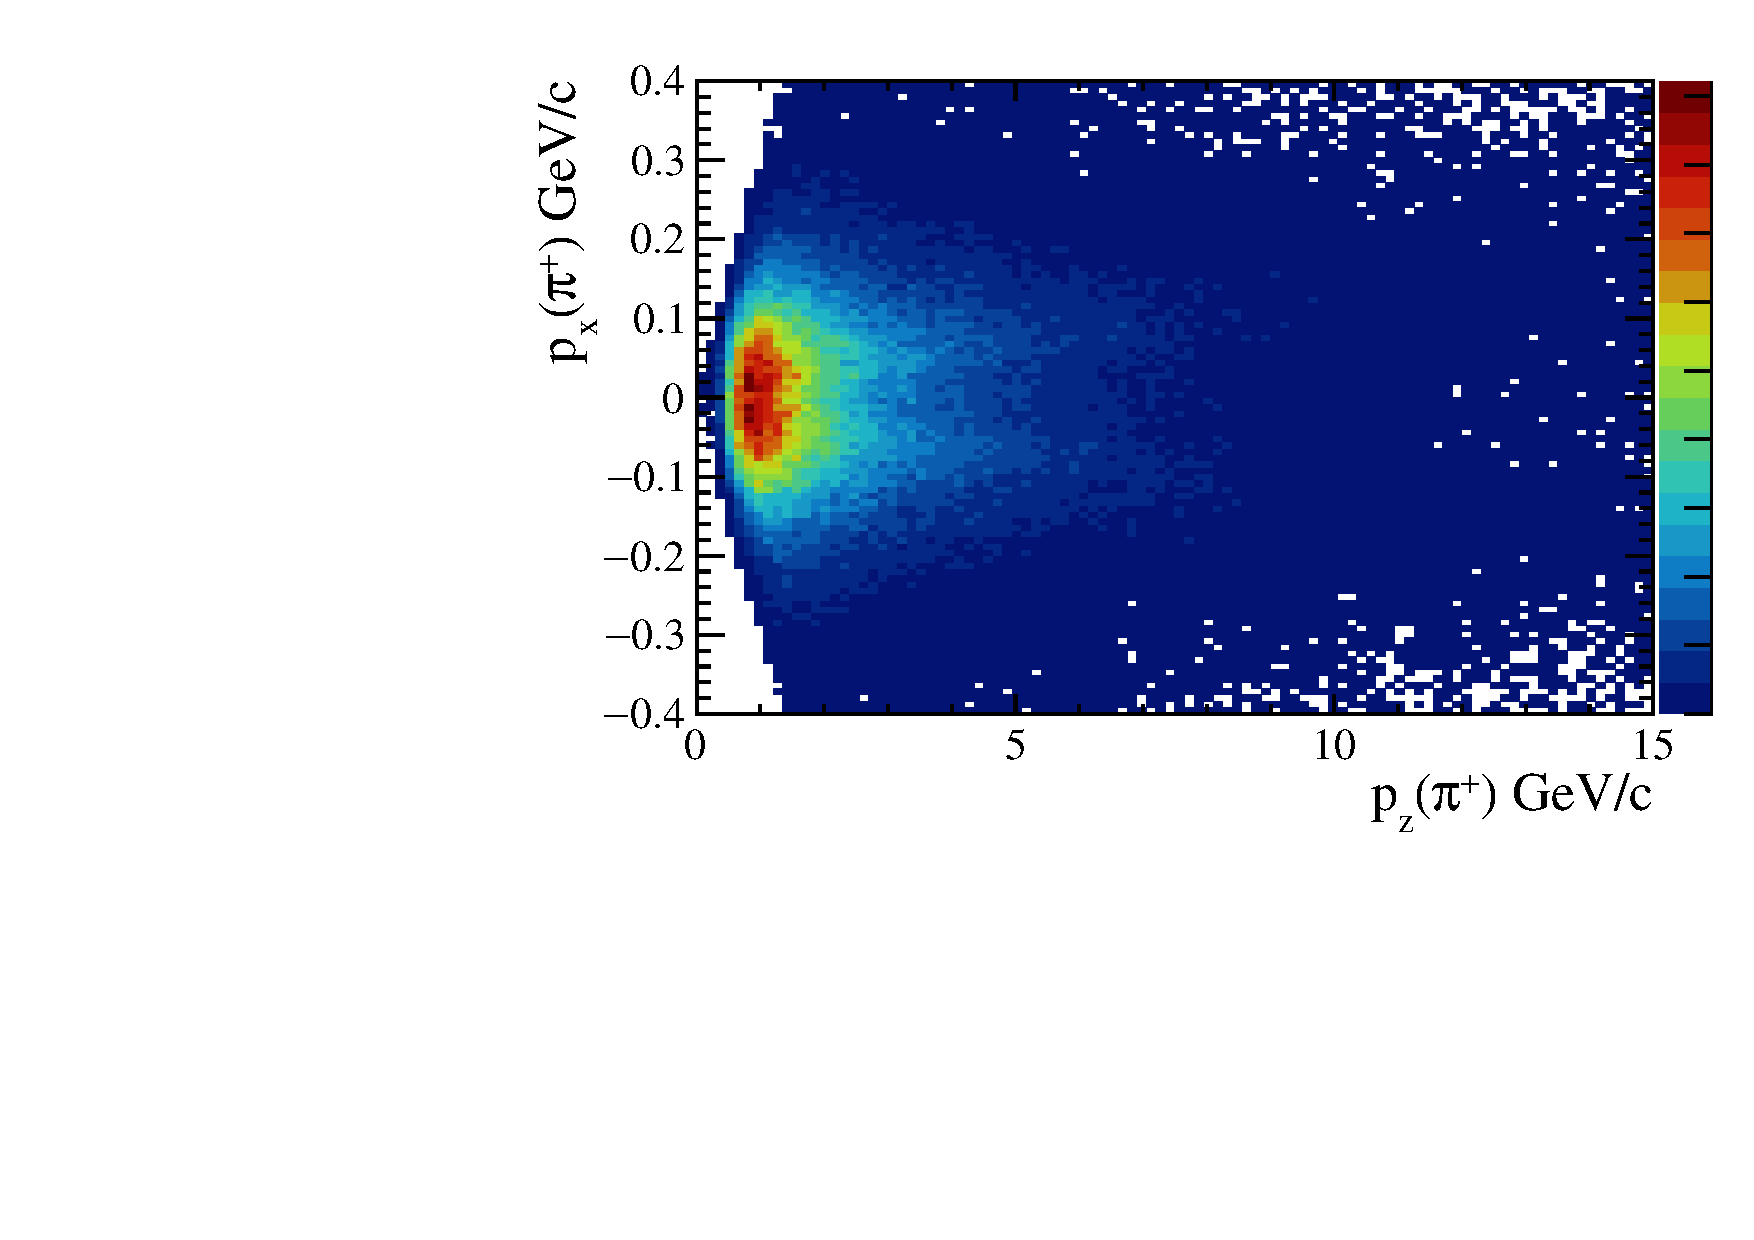
\includegraphics[width = 0.9\textwidth]{../work/RapidSimAnalysis/MomentumDependence/Plots/KK_Dst_PXPZ_Positive.pdf}
                  \end{figure}
            
            \column{0.5\textwidth}
                  \begin{figure}
                        \centering
                        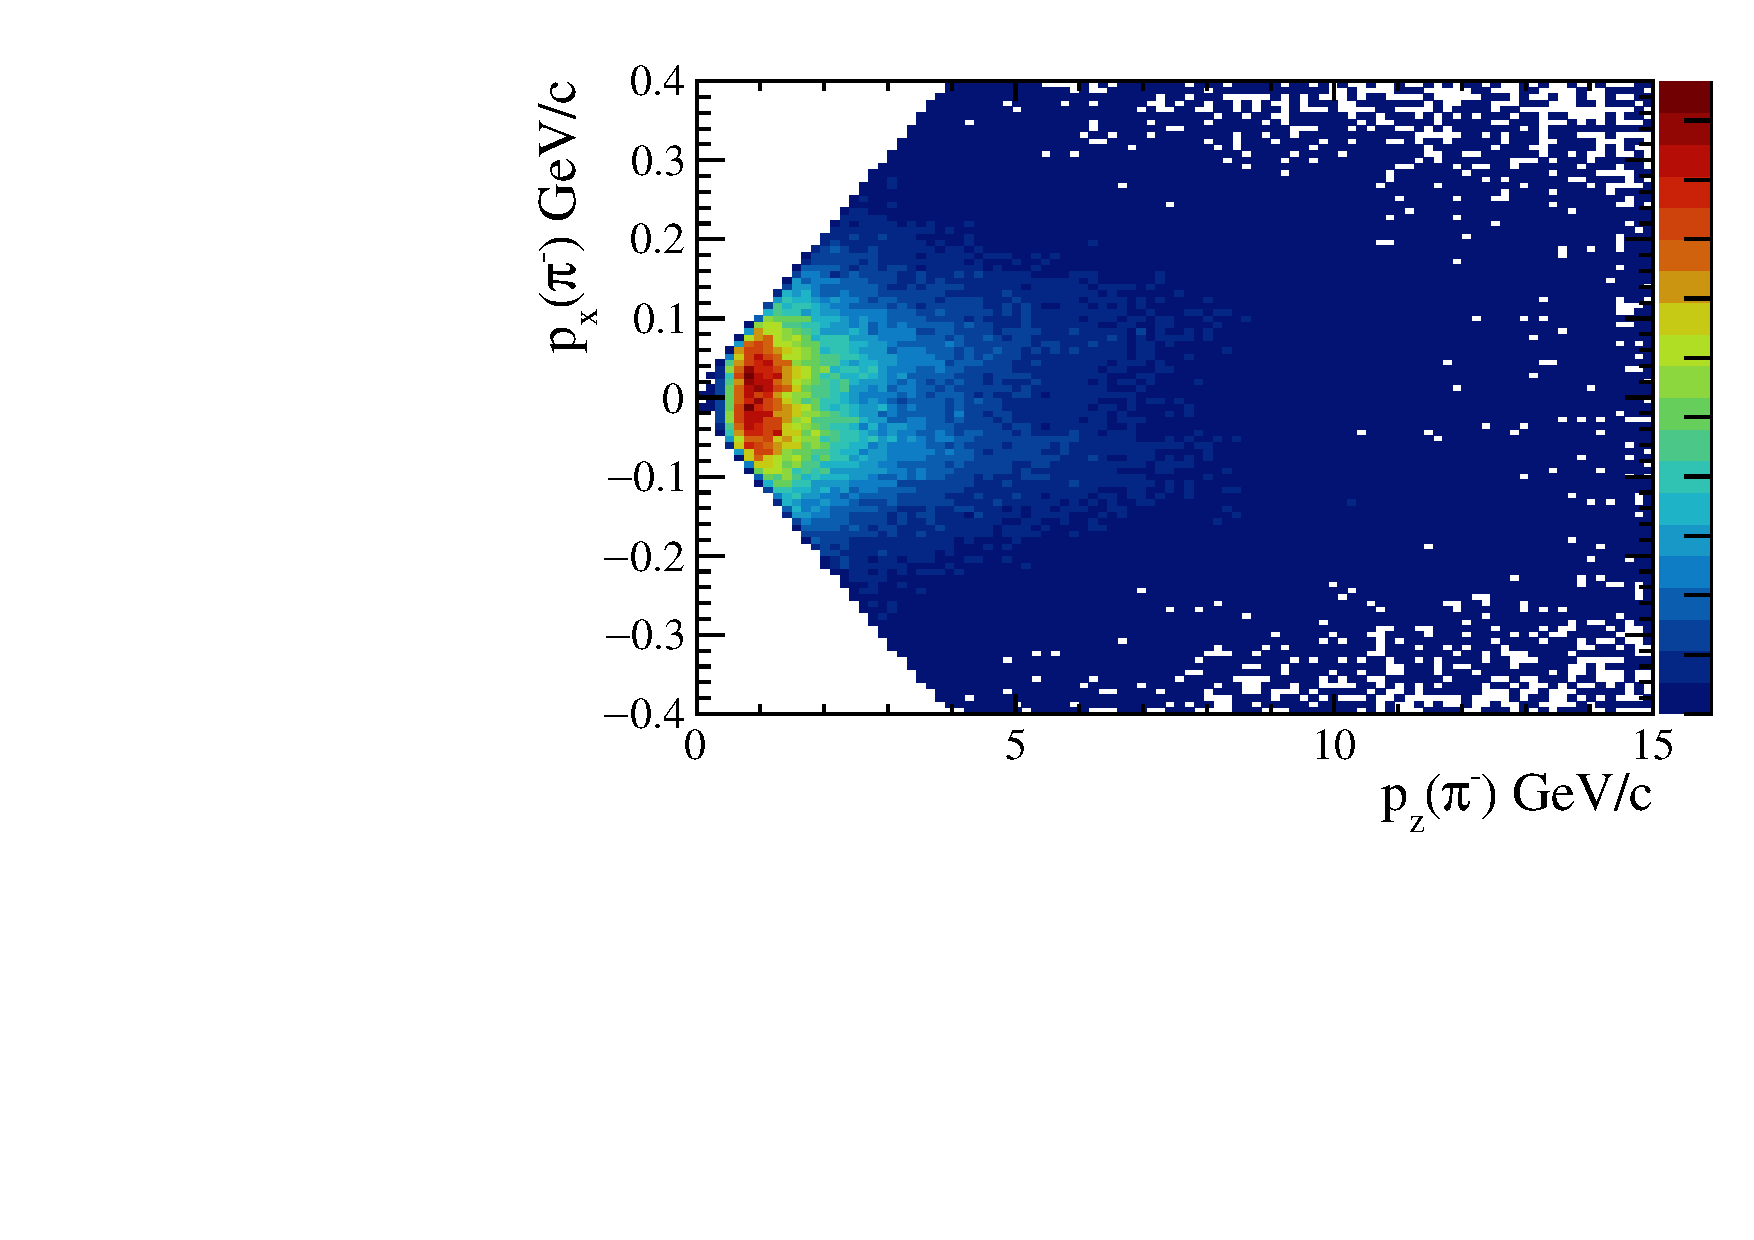
\includegraphics[width = 0.9\textwidth]{../work/RapidSimAnalysis/MomentumDependence/Plots/KK_Dst_PXPZ_Negative.pdf}
                  \end{figure}

      \end{columns}
      \begin{itemize}
            \item The $\pi_s^+$ sector is left unchanged
            \item The $\pi_s^-$ sector has a detection asymmetry to simulate the LHCb plots
      \end{itemize}
\end{frame}

\subsection{Weighting function}
\begin{frame}
      \frametitle{\insertsubsectionhead}
      \begin{itemize}
            \item We calculate the weighting function before and after the detection asymmetry
      \end{itemize}
      \begin{columns}
            \column{0.5\textwidth}
                  \begin{figure}
                        \centering
                        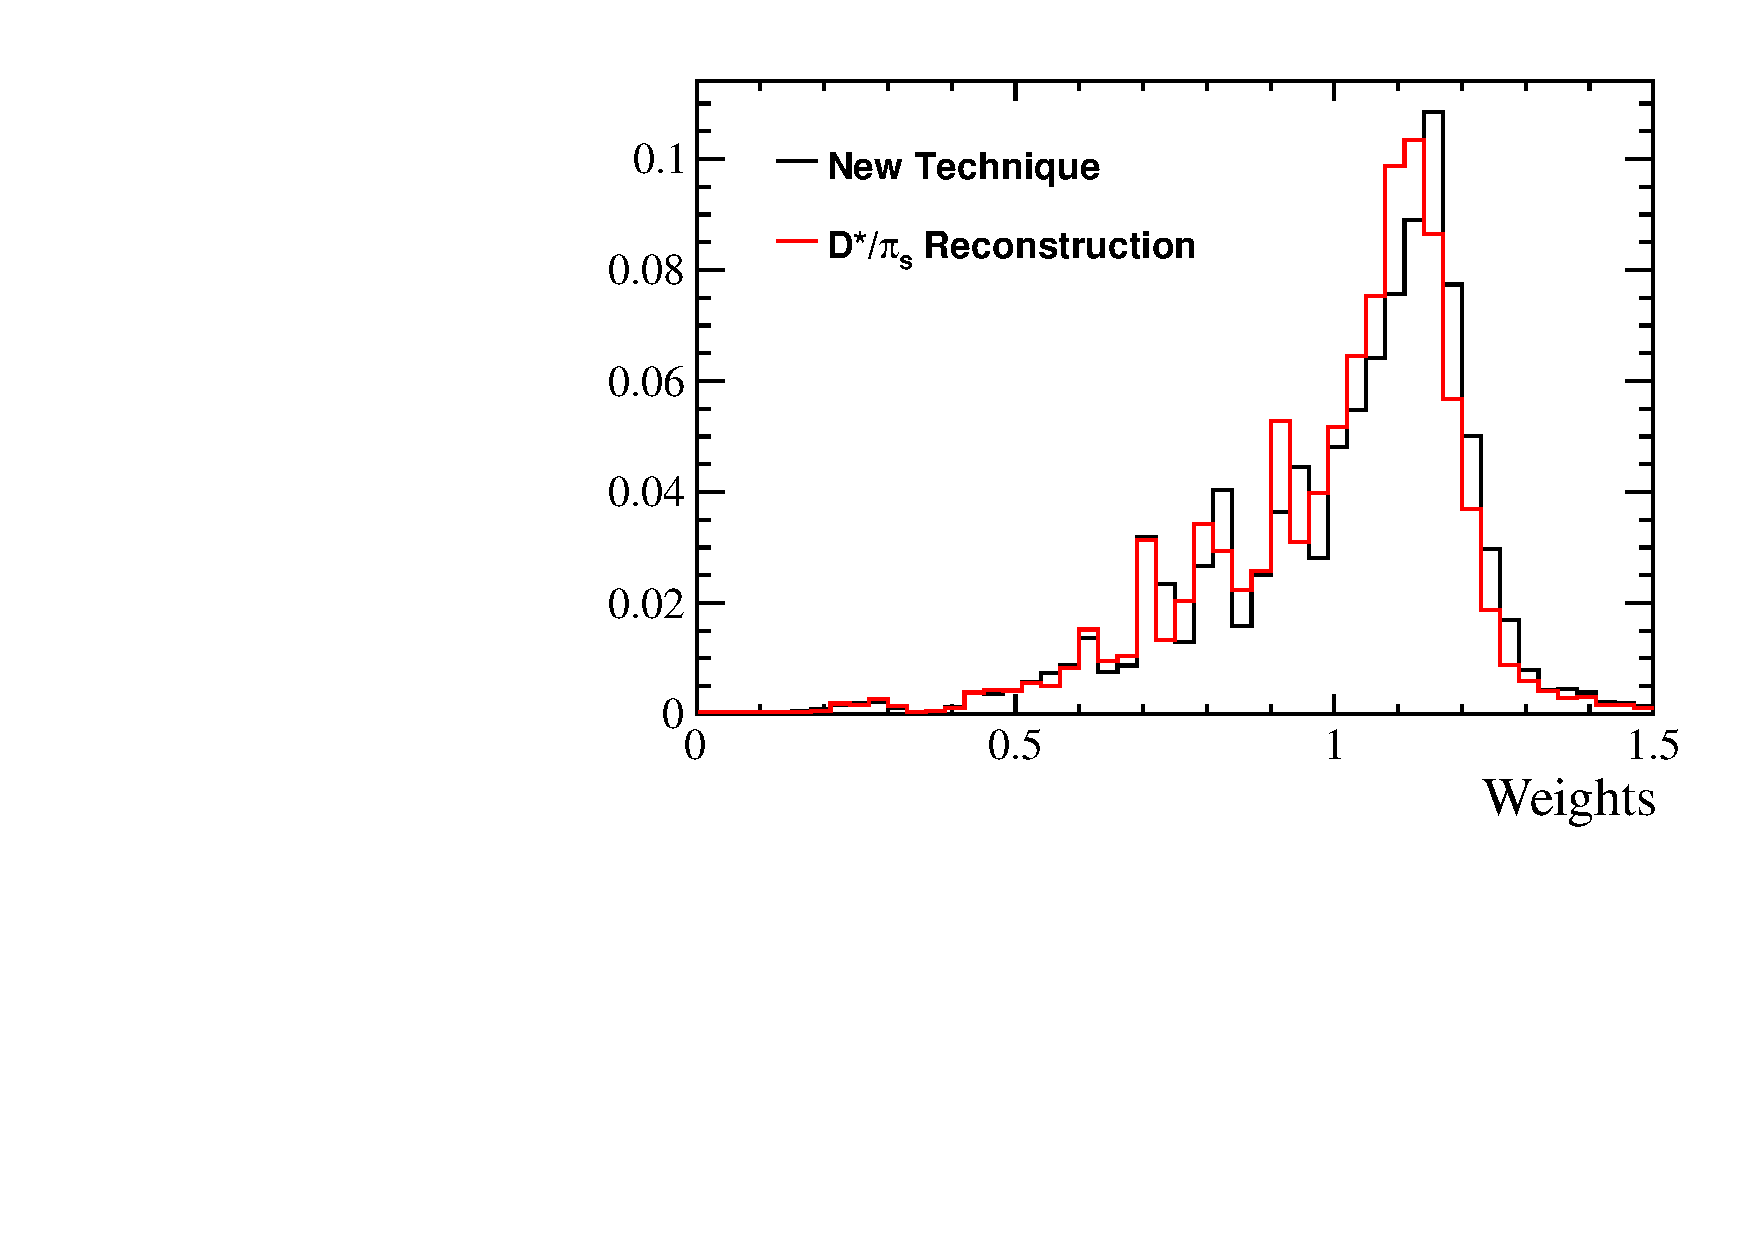
\includegraphics[width = \textwidth]{../work/RapidSimAnalysis/NewWeightingFunction/Plots/WeighsBeforeAfter.pdf}
                  \end{figure}
            \column{0.5\textwidth}
                  \begin{itemize}
                        \item Slight difference between the two
                        \item How will the final results change?
                  \end{itemize}
      \end{columns}
\end{frame}

\begin{frame}
      \LARGE
      \centering
      Thank you for your attention!

      Questions?
\end{frame}
\end{document}